\section{Lec 10}


\subsection{$\emph{AGD}$ in Strongly Convex Cases}

$\emph{AGD}$ for $L$-smooth convex functions was discussed in the last lecture.

Here we consider $\emph{AGD}$ for $L$-smooth and $m$-strongly convex functions.

We use constant parameters
\[
\alpha_k = \frac{1}{L},
\qquad
\beta_k = \frac{\sqrt{L} - \sqrt{m}}{\sqrt{L} + \sqrt{m}},
\quad \forall k.
\]
This implicitly assumes $L>m$, where $L$ is the upper bound on the curvature and $m$ is the lower bound.

\begin{theorembox}
For an $L$-smooth and $m$-strongly convex function $f$ with minimizer $\bm x^*$, accelerated gradient descent with
\[
\alpha_k = \frac{1}{L},
\qquad
\beta_k = \frac{\sqrt{L} - \sqrt{m}}{\sqrt{L} + \sqrt{m}}
\]
satisfies
\[
f(\bm x^k) - f(\bm x^*)
\le
\left(1 - \sqrt{\frac{m}{L}}\right)^k
\left[
f(\bm x^0) - f(\bm x^*) +
\frac{m}{2}\bigl\|\bm x^0 - \bm x^*\bigr\|^2
\right].
\]
In particular, the method has \textbf{linear convergence}.
\end{theorembox}

This rate is faster than standard $\emph{GD}$, whose linear rate is
\[
\left(1 - \frac{m}{L}\right)^k.
\]
Hence, in the strongly convex case, $\emph{AGD}$ provides a significant improvement over $\emph{GD}$.


When $\dfrac{m}{L} \ll 1$, the \emph{convex} (non-strongly-convex) version of $\emph{AGD}$ may actually perform better for moderate $k$.  
A version of $\emph{AGD}$ that simultaneously attains both the strongly-convex and merely-convex bounds is well known and can be found in Nesterov's book.

\medskip
\textit{Note.} Conjugate Gradient is not covered in this lecture.

\subsection{Aside on Programming}

From Problem Set 2:

\begin{verbatim}
function huber_minimize(A, y, tol, x0, L, tau)

  while ...
    % ← Gradient Descent main loop
    evaluate huber gradient

end
\end{verbatim}

We would like to separate the Huber-specific code from the general $\emph{GD}$ algorithm.

\textit{Tendency.}
\begin{itemize}
  \item The \texttt{gradfunc()} represents the gradient of the objective, and it internally depends on \texttt{A}, \texttt{y}, and \texttt{tau}.
\end{itemize}

\begin{examplebox}
\textbf{(Huber gradient wrapper.)}
\begin{verbatim}
function g = huber_grad(x)
    % Evaluate Huber gradient
end
\end{verbatim}

Then, we pass \texttt{huber\_grad()} as the first argument of the optimizer:
\begin{verbatim}
function xopt = agd(gradfunc, x0, tol, L)
\end{verbatim}
\end{examplebox}

Now we have a call chain:
\begin{center}
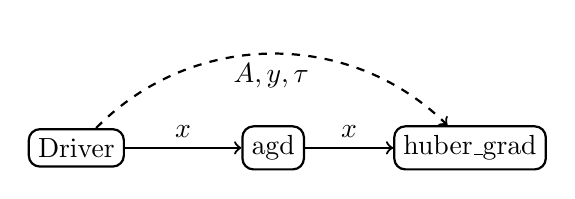
\begin{tikzpicture}[node distance=2.5cm, ->, thick]
  \node (D) [draw, rectangle, rounded corners] {Driver};
  \node (G) [draw, rectangle, rounded corners, right of=D] {agd};
  \node (H) [draw, rectangle, rounded corners, right of=G] {huber\_grad};
  \draw (D) -- node[above] {$x$} (G);
  \draw (G) -- node[above] {$x$} (H);
  \draw[dashed] (D) to[bend left=45] node[below] {$A, y, \tau$} (H);
\end{tikzpicture}
\end{center}

However, \texttt{huber\_grad()} needs access to \texttt{A}, \texttt{y}, and \texttt{tau}, which are defined in \texttt{driver()} and not directly passed to it.


\textit{Old solutions.}
\begin{enumerate}
  \item \textbf{Global variables.}\\
  Store \texttt{A}, \texttt{y}, and \texttt{tau} in global variables known to both \texttt{driver()} and \texttt{huber\_grad()}.\\
  \emph{Risk:} name clashes, hard to debug.

  \item \textbf{Opaque parameter struct.}\\
  Pass an additional argument \texttt{params} to \texttt{agd()}.  
  The \texttt{driver()} packs \texttt{A}, \texttt{y}, and \texttt{tau} inside, and \texttt{huber\_grad()} unpacks them.\\
  \emph{Risk:} troublesome packing and unpacking, error-prone.
\end{enumerate}


\textit{Modern solutions.}
\begin{enumerate}
  \item \textbf{Inner function.}
\begin{verbatim}
function driver
    A = ...;
    y = ...;
    tau = ...;

    function g = huber_grad(x)
        % uses A, y, tau
    end

    xopt = agd(@huber_grad, x0, tol, L);
end
\end{verbatim}

  \item \textbf{Anonymous function (closure / lambda).}
\begin{verbatim}
function g = huber_grad(x, A, y, tau)
    % Evaluate Huber gradient
end

function driver
    A = ...;
    y = ...;
    tau = ...;

    gradfunc = @(x) huber_grad(x, A, y, tau);
    xopt = agd(gradfunc, x0, tol, L);
end
\end{verbatim}
\end{enumerate}


\textit{Note.} For Problem Set 3, use one of these two modern methods (inner or anonymous functions). Or, besides the two modern methods, can also use \emph{objects} to represent functions in Problem Set 3.

\subsection{Binary Classification}

Given $N$ data points $(\bm a_1, y_1), \dots, (\bm a_N, y_N)$ with $y_i \in \{+1, -1\}$ and $\bm a_i \in \R^n$ for all $i$, we want to learn a vector $\bm x$ such that
\[
\bm a_i^\top \bm x > 0 \text{ for } y_i = +1,
\qquad
\bm a_i^\top \bm x < 0 \text{ for } y_i = -1.
\]
Such an $\bm x$ defines a \textbf{linear classifier}.


We can extend this idea to nonlinear classifiers by enriching the feature representation of each $\bm a_i$.

\begin{examplebox}
\textbf{(Feature mapping.)}
One approach is to use monomial features (as in Problem Set 1) to construct a higher-dimensional feature vector for each $\bm a_i$, on which a linear classifier is then learned.
\end{examplebox}

To allow the classifier to represent a hyperplane not passing through the origin, we can append a constant $1$ to each $\bm a_i$, which is known as the \textbf{padding trick}.

\subsubsection{Logistic Regression}

We say the data is \textbf{linearly separable} if there exists $\bm x$ such that  
$\bm a_i^\top \bm x > 0$ for $y_i = +1$ and $\bm a_i^\top \bm x < 0$ for $y_i = -1$.

Define
\[
\varphi(t) \defeq
\begin{cases}
1,  & t > 0,\\
-1, & t < 0.
\end{cases}
\]

Define
\[
L \defeq
\prod_{i: y_i = 1} \dfrac{\varphi(\bm a_i^\top \bm x) + 1}{2}
\prod_{i: y_i = -1} \dfrac{-\varphi(\bm a_i^\top \bm x) + 1}{2}.
\]
Then $L = 1$ if all points are correctly classified, and $L = 0$ otherwise.

One idea is to find the classifier by maximizing $L$ as a function of $\bm x$.  
This fails if the data points are not linearly separable, since $L$ then cannot achieve $1$.


To fix this, redefine $\varphi$ (since the original one is discontinuous):
\[
\varphi(t) \defeq \frac{-1 + \mathrm e^t}{1 + \mathrm e^t}.
\]

Use the same formula for $L$, but with this new $\varphi$.  
(It is easier to work with $\ln L$.)

\[
\max_{\bm x}
\left[
\sum_{i: y_i = 1} \ln\bigl(\varphi(\bm a_i^\top \bm x) + 1\bigr)
+ \sum_{i: y_i = -1} \ln\bigl(-\varphi(\bm a_i^\top \bm x) + 1\bigr)
\right].
\]

This is called \textbf{Logistic Regression}.


Compute the logarithmic terms:
\[
\begin{aligned}
\ln(\varphi(t) + 1)
&= \ln\left(\frac{-1 + \mathrm e^t + 1 + \mathrm e^t}{1 + \mathrm e^t}\right)
= \ln\left(\frac{2 \mathrm e^t}{1 + \mathrm e^t}\right)
= \ln\left(\frac{2}{1 + \mathrm e^{-t}}\right)
= \ln 2 - \ln(1 + \mathrm e^{-t}),
\\[0.4em]
\ln(-\varphi(t) + 1)
&= \ln 2 - \ln(1 + \mathrm e^{t}).
\end{aligned}
\]

Dropping additive constants, logistic regression becomes
\[
\min_{\bm x}
\left[
\sum_{i: y_i = 1} \ln\bigl(1 + \mathrm e^{-\bm a_i^\top \bm x}\bigr)
+ \sum_{i: y_i = -1} \ln\bigl(1 + \mathrm e^{\bm a_i^\top \bm x}\bigr)
\right].
\]

\begin{factbox}
The logistic regression objective
\[
\bm x \;\mapsto\;
\sum_{i: y_i = 1} \ln\bigl(1 + \mathrm e^{-\bm a_i^\top \bm x}\bigr)
+ \sum_{i: y_i = -1} \ln\bigl(1 + \mathrm e^{\bm a_i^\top \bm x}\bigr)
\]
is convex and $L$-smooth (for some $L$ depending on the data).
\end{factbox}


However, if the data is linearly separable, then the problem has \emph{no} minimizer, since any separating $\bm x$ can be scaled arbitrarily large.  
Gradient descent then drives $\|\bm x\|\to\infty$.

To limit this, add a \textbf{regularizing term}:
\[
\min_{\bm x}
\frac{1}{N}
\left[
\sum_{i: y_i = 1} \cdots
+ \sum_{i: y_i = -1} \cdots
\right]
+ \frac{\gamma}{2} \|\bm x\|^2.
\]
Here $\gamma>0$ is the \textbf{regularization parameter}, and this is known as $\ell_2$ regularization.

Later we will cover $\ell_1$ regularization.


Now we can minimize this regularized objective using $\emph{GD}$ or $\emph{AGD}$.

But what if $N = 10^9$?  
Gradient evaluation is very expensive, and not all data points are needed to obtain a good $\bm x$.

\subsubsection{Stochastic Gradient Descent $\emph{SGD}$}

Rewrite the regularized objective as
\[
\mathbb{E}\!\left[
l(\bm a, y; \bm x)
\right]
+ \frac{\gamma}{2} \|\bm x\|^2,
\]
where the expectation is over a random data pair $(\bm a,y)$ drawn uniformly from the dataset, and $l$ is the logistic loss for a single sample.

In $\emph{SGD}$, instead of using the full gradient of the expectation, we randomly select one data pair $(\bm a_i, y_i)$ and compute the stochastic gradient
\[
\nabla_{\bm x}
\left[
l(\bm a_i, y_i; \bm x)
+ \frac{\gamma}{2} \|\bm x\|^2
\right].
\]

At each iteration, a new random pair is chosen. This yields much cheaper iterations and scales to very large datasets.
